% !TeX spellcheck = en_US
%\chapter{Design} 
%\section{Design of the data access}
%\section{Filters}

%=======================================================================
\chapter{Design of an information system for support of forensic audit}\label {Design}
%\komentar{
%vsechno o tom systemu jako takovem, ale tak, aby to navazovalo na predchozi...?
%
%prostredi webu + silne zabezpeceni, reporty, export, pdf\\
%maly informativni obrazek, ktery poskytne uzivateli informaci o tom, co se stalo\\
%! pripojit pripady uziti vcetne zavislosti\\
%
%jedna se o aplikaci, ktera provazi celym projektem (zadanim) forenzniho auditu. sice existuji i jiny nastroje pro podporu takovychto projektu, ale projekt ma useky a nam jde o integraci porizenych vysledku
%
%}

%=======================================================================

This chapter deals with the design of the information system. Approaches to the implementation of requirements on the system stated in \ref{Requirements} are described here. We also provide a discussion about technologies useful for implementation and the description is accompanied with diagrams demonstrating the design. 

\section{Application}

The architecture of our application will be based on two fundamental parts. One of them will be collecting the data we will use and the other will display them to the user. From now on we will call this the \name{Collector} and the \name{Displayer}. This is a useful division because it simplifies the design and also keeps it easier to maintain. The aim of the \name{Collector} will be to transform the data from various sources to some generic format for easier manipulation.

There are numerous types of sources of data that can be used as evidence in forensic audit. The data can differ in inner structure and also in the content. Examples of this diversity are IM messages, pictures, GPS coordinates, audio-video files,emails logs of network activities, public information from social sites and internal company management or accounting system.

Ideally our system is able to work with all of them, however we exclude pictures and the audio-video material from these sources because this material does not need visualization. Nevertheless, our system needs to be able to process the information this type of material contains, in case that it could be converted to the basic structure of our application, which will be described later. The task to provide this functionality is assigned to the \name{Collector}.

Each of the previously mentioned type of source of data is somehow specific. Thus we need a specific solution for each one of them. This is an ideal job for a plug-in architecture. 

\begin{figure}[!h]
    \centering 
    \epsfysize=60mm 
    \epsffile{./img/diagrams/Architecture.eps} 
    \caption{Architecture of the application}\label{Architecture}
\end{figure}

Plug-in is a piece of software that does not work separately, it only extends the functionality of the application. The application usually provides an Application Programming Interface (API) so that the plug-in extension could communicate with the application properly. In case of this application it means that for each source of data there will be a specific plug-in. each plug-in will be made specifically for the format of the source file. The purpose of the plug-in will be to read the source files and prepare the data for the \name{Collector}. The collector than saves it to the database. Finally the \name{Displayer} will access the database and provide the visualization of the case.

\begin{figure}[!h]
    \centering 
    \epsfysize=60mm 
    \epsffile{./img/diagrams/Plug-ins.eps} 
    \caption{Collector}\label{Collector}
\end{figure}

\subsection{Database}
\paragraph{Entity \name{Event}}
The database model of our application is based on a entity called \name{Event} and several other entities. The Primary unique identification number (UID) of \name{Event} is Integer ID. It also consists of one mandatory time-stamp that indicates the time this event occurred or the time of the start if the event was long-lasting. We need to distinguish between one-time events and longer lasting ones so in there is a mandatory boolean attribute \name{LongLasting} playing the role of a flag. If this attribute is true, another time-stamp attribute indicating the end of the \name{Event} is to be filled in. 

\begin{figure}[!h]
    \centering 
    \epsfysize=180mm 
    \epsffile{./img/datamodel/logical.pdf} 
    \caption{Logical model of the database}\label{Logical}
\end{figure}

\paragraph{Entity \name{Event\_Detail}}
We have prepared a entity \name{Event\_Detail} in case there would be some other details concerning the \name{Event}. This entity is in a 1:n relationship with \name{Event}. It means, that if we will need, there can be more details concerning \name{Event}. \name{Event\_Detail} has only one mandatory attribute called \name{Description}, that is prepared for 128 characters of text. For \name{Event} the relationship with \name{Event\_Detail} is optional, however, for \name{Event\_Detail} it is compulsory and the ID of \name{Event} is its foreign key. 

\paragraph{}
The data we expect to use as a source should also contain information about the subject causing the event. For the subject we have a special model. Before describing it, let us explain why we need it. We cannot be sure what sources and what information concerning the subjects we will get. Our source files should primarily contain logs of various kinds of activities, not only logs of one subject. Because of this we cannot easily connect actual person with events. The identifier of the subject can be of different kind in different sources. For example while email clients are identified by email address, e.g. character stings, IM users are identified by integer ID, nickname or even e-mail address. However this identifier is definitely not the same as the bank account number. Still ne subject may be identified by any number of any of these ways.

For simplicity we decided not to deal with merging these various accounts of one subject in the database as it would increase complexity greatly. This will be done later by the \name{Displayer}. 

\paragraph{\name{Participant}}
In our database model we now establish the \name{Participant} entity. The primary key of this entity is an integer ID and next attribute is optional a 36-char-long \name{Name}. This attribute is prepared for the case that the name of the participant would be stated in the source. For actual information about the source we prepare two extra mandatory attributes. The first, called \name{type}, is designed to inform about the source of data the particular information came from. The second one is called \name{alias} and it is an array of 32 characters prepared to store the original identifier of the participant.

The \name{Participant} entity contains two other entities called \name{Active} and \name{Passive}. Each one of them has the entity \name{Participant} as its superstructure. The relationship between \name{Participant} and \name{Event} is arranged via these two entities. Both these relationships are of m:n type. The only difference between them is that  for the \name{Event} entity the relationship with \name{Active Participant} is compulsory whereas with \name{Passive Participant} is optional. 

This model enables \name{Events} to have more \name{Participants}, but forces the \name{Event} to have at least one \name{Active Participant}.


\begin{figure}[!h]
    \centering 
    
    \epsfysize=180mm 
    \epsffile{./img/datamodel/relational.pdf} 
    \caption{Relational model}\label{Relational}
\end{figure}

\subsection{\name{Collector}} 

The next section focuses on the \name{Collector} part of the application. Before we start let us mention that the main purpose of the \name{Collector} is to provide an interface for inserting data to the database and managing the plug-ins that translate the source format to our format (based on the event structure). The \name{Collector} has its own GUI that enables the user to choose from existing plug-ins or add new ones. The GUI saves the configuration to a configuration file and then hands it over to the \name{Collector} back end. The \name{Collector} provides the user the possibility of selecting and running the plug-ins. Each plug-in has its own GUI so that the user can specify any information needed for them to run of the plug-in (such as the path to a file with the source material). 

The \name{Collector} also manages the plug-ins added to the application. It means that it has a configuration file where all paths to the plug-ins are saved together with short clear description of the source. %\todo{} (tady jsem nejak prestala) \todo{}

The key API that the \name{Collector} provides to the plug-in is basically the access to the database. %It might be a bit risky to provide the access to the database to a unknown piece of software.
Plug-ins load data into the tables and the \name{Collector} pushes the data into the database. Each plug-in only processes the source file to the data model, create a SQL query and fill in the database. Note, that this application is expected to process data of a text character only. The application is not prepared for mining data from files of multimedia character unless the content is described in a structured text containing the date and some information identifying the related subject.

\begin{figure}[h]
	\begin{center} 
	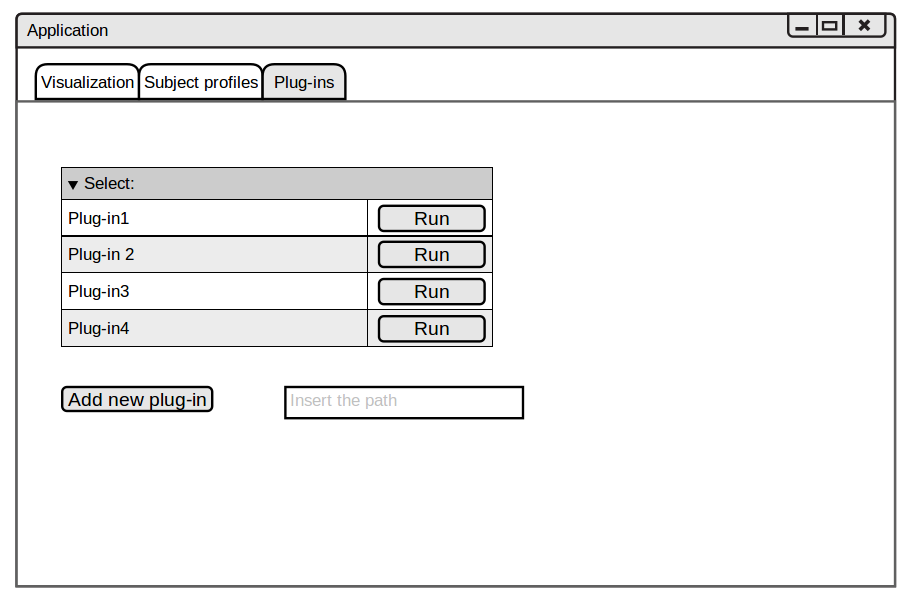
\includegraphics[width=1.0\textwidth]{./img/GUI/Plug-ins.png}
	\end{center}
	\caption{Graphical user interface of the plug-in manager}\label{plug-ins}
\end{figure}

\subsection{\name{Displayer}}

The main purpose of the displayer is to visualize the data saved in the database. To be able to do this, it is necessary at first to deal with the problem of multiple \name{Participants} in the database that all represent the same \name{Subject}. We can overcame this obstacle easily by creating a table for \name{Participant} unification to \name {Subjects}. However, because of the essence of the data we are working with and the general purpose of our application, we cannot try to guess which \name{Participants} belong together. Therefore there is a special form helping the auditor unify them to subjects. 

\begin{figure}[h]
	\begin{center} 
	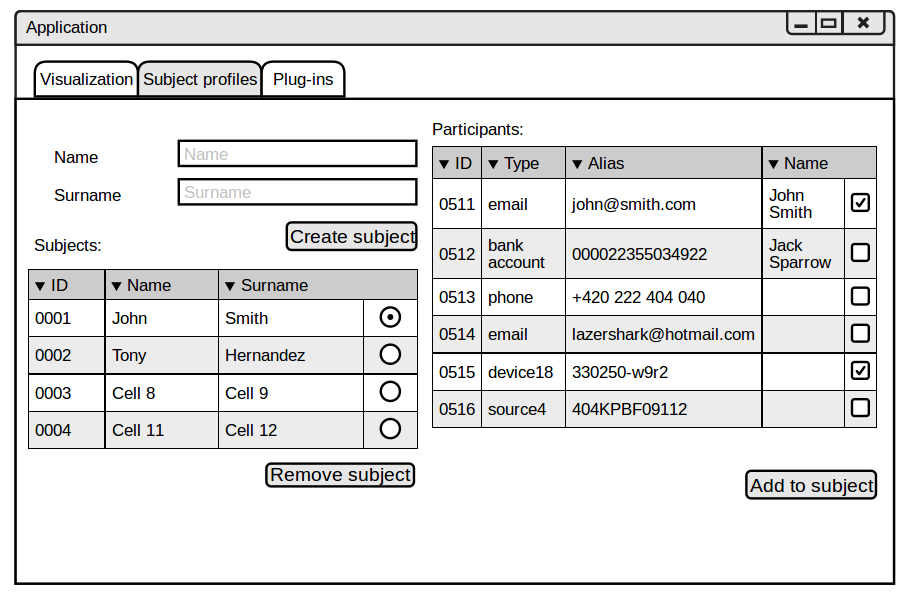
\includegraphics[width=1.0\textwidth]{./img/GUI/Subject_profiles.png}
	\end{center}
	\caption{Form for unifying \name{Participants} to Subjects}\label{form}
\end{figure}

Sample form is shown in the figure \ref{form}. In the left table there is a list of existing subjects. The user can add new subjects easily by filling in the name and surname and by clicking on the "Create subject" button. Auditor can also remove a subject by clicking on "Remove subject" button or edit name or surname of subject by clicking into the table. The \name{Displayer} creates a table containing the information about this mapping. When replaying the displayer uses this information to identify the correct events for each subject. The data model shown in picture \ref{model-displayer} indicates that each \name{Subject} can have many \name{Participants}, but each \name{Participant} can have only one \name{Subject}.

\begin{figure}[!h]
    \centering 
    
    \epsfysize=40mm 
    \epsffile{./img/datamodel/subj-participant.pdf} 
    \caption{The relation between \name{Subject} and \name{Participant}}\label{model-displayer}
\end{figure}

Now we can focus on the most important function of the application. We have a background for the visualization in the above modeled database. In the initialization phase the \name{Displayer} generates names of all the known \name{Subjects} and places a checkbox next to each one of them. The state of the checkbox decides whether we want to include the related \name{Subject} in the visualization. 

In the next step the \name{Displayer} enters proper SQL query. IDs of the subjects are replaced by the entire group of \name{Participants}. We then search in the database for all \name{Events} whose starting time is later than the date selected in the visualization tab and at the same time the some of the \name{Subjects} takes part in it. We also search for  \name{LongLasting} \name{Events} that end after the selected time frame. The result of the  selected  \name{Events} is then replayed by time. 

The process of replaying has a small obstacle concerning various animations in different cases. These differences are:
\begin{enumerate}
\item If \name{Subject} does not take part in current \name{Event} it is displayed as a red dot.
\item If \name{Subject} takes part in a \name{Event} alone it is displayed as a green dot.
\item If \name{Subject} causes an \name{Event} the color of the active \name{Subject} is green and a arrow aiming at the passive \name{Subject} is displayed. 
\item If more \name{Subjects} actively participate in one \name{Event} they are all displayed in green color and a line connecting them together is displayed between them. 
\end{enumerate}

 The solution for the first and second case is trivial. The color of all \name{Subjects} is red by default so only if we run into a \name{Event} where a subject takes a part we change the color for a constant period of displayed time. If the \name{Event} has a passive \name{Participant}, as described in third case, we draw an arrow from the active to the passive \name{Subject}. Similarly, if the \name{Event} has more \name{Active Participants} the line between them is drawn.  
 
 All these situations are easily recognizable using SQL queries. 
% 
% 
%\todo{} The inner design of the \name{Displayer}
%It was already mentioned that the \name{Displayer} acquires \name{Events} for replaying using SQL queries. There is only one aspect left to describe and it is the inner design of the \name{Displayer}. To be able to run the \name{Displayer} needs the table mapping  \name{Participants} to \name{Subjects}. We recommend not to save this table in the database, but rather store it in memory for faster accessibility. The user needs to follow only several units of subjects in the animation. \todo
% 
 
 
\chapter{Discussion} \label{Discussion}

%popis rozdil mezi flatfile a databazi externi vs embeded
\paragraph{Database} %\todo{}

We recommend to use the Oracle database. The main reason is that it is one of the fastest and safest relational databases. If it was necessary since it is a relational database it could be replaced for any other relational database and the Oracle Data Modeler is also very easy to use, we have already some good experience with it. 

\paragraph{Open Database Connectivity}
Open Database Connectivity (ODBC) is a standardized software API that enables the access to database servers. The aim of ODBC is to provide an access independent on programming language, operating system or the database system. We recommend to use this technique while implementing this application. 

We would also recommend to use the C/C++ programming language. The Qt library can be used for implementation of the GUI of this program.

\paragraph*{Further improvement}
Follow-up work would definitely include the implementation of the designed application, testing and hands-on experience with real data.
Mainly real-world use will show deficiencies, if any, and provide necessary insight for modifications and extensions.


%paragraph{Flat File} 
%
% flat file database is the simplest form of database. It stores data in a plain text file \cite{x2}.%http://techterms.com/definition/flatfile 
%here is one record per line. Fields in each line are separated by 
%elimiters such as tabulator or comma. In this model data are stored in multiple files, however these 
%iles are not linked, so the data may be repeated in several files. The advantage of this kind of database is the simplicity.
%t can also be easily transformed into most other databases. One disadvantage is performance drop for large databases, which may 
%equire linear walk for random access, thus loading unnecessary data into memory. Another disadvantage is 
%hat a flat file usually requires writing and debugging custom code, which may extend the time to develop the application.
%t is not a widely used type of a database. 
%
%
%paragraph{SQL database management system}
%oday's SQL databases provide reliable data storage with the widest feature sets, powering some of the biggest companies.Their advantages include large feature sets and independence on the applications that use them and they are well documented and easy to first setup thanks to them being so commonplace
%n the other hand they are criticized for their lack of performance, bloated specifications and difficult optimizations which are required when their aforementioned lack
%f performance shows itself.
%
%xamples include MySQL, PostgreSQL and IBM DB2.
%
%paragraph{NoSQL database} %<-tohle je nejrychlejsi
%
%oSQL databases handle data based on different models than relational databases. Their data model is more tightly coupled with the needs of the application.
%hese databases may or may not use general query language to access data (NoSQL may be also interpreted as Not-only-SQL), but they particularly shine when they don't and instead the application uses their API
%o access the data directly.
%
%heir performance is often unmatched, but may be more difficult to use due to their lack of powerful tools the SQL offers.
%
%here are several methods to categorize NoSQL databases, all with diverse classes and subclasses. Because of the variability of the methodologies and overlays it is problematic to acquire and preserve an indication of non-relational databases. Yet, a basic arrangement is based on data model. A few examples in each group are:
%
%begin{itemize}
%item \textbf{Graph:} InfiniteGraph, OrientDB
%item \textbf{Multi-model:} ArangoDB, Alchemy Database
%item \textbf{Column:} Druid, Hbase
%item \textbf{Document:} Clusterpoint, OrientDB
%item \textbf{Key-value:} Oracle NoSQL Database, Dynamo, LMDB, LevelDB
%end{itemize}
%
%
%paragraph{NewSQL database} %<-tohle by asi bylo idealni
%he NewSQL database is a type of modern relational database management system that attempts to combine the speed and efficiency of NoSQL databases while 
%etaining the relational database model.
%
%mong NewSQL databases may be included these: H-Store, Clustrix, VoltDB, MemSQL.
%
%he NewSQL database will be more appropriate for storing our data in terms of its speediness and functionality for forensic investigation, as compared to the rest of the database techniques mentioned above. Especially more complex operations on data would be missed on databases without SQL support.
%
%
%








